\documentclass[11pt]{article}
\usepackage[margin=23mm]{geometry}
\usepackage{amsmath,amssymb,booktabs,graphicx,hyperref}
\hypersetup{colorlinks=true,urlcolor=blue,linkcolor=blue}
\renewcommand{\topfraction}{0.95}
\renewcommand{\textfraction}{0.05}
\renewcommand{\floatpagefraction}{0.85}
\newcommand{\Ha}{H$\alpha$}
\newcommand{\Lb}{Ly$\beta$}
\title{H-alpha transport: geometry, velocity and photon recycling}
\author{exojax-escape investigation}
\date{26 November 2026}
\begin{document}
\maketitle
\section{Question and scope}
The physical atmosphere used in PRs 12 and 13 produces too little blue-peak
contrast and an insufficient central depression in the observed profile.
Fixed-state source-function perturbations motivate asking whether radiation
from inner emitting layers is too strongly coupled to the upper atmosphere.
Here three parallel calculations test finite geometry, differential velocities,
and H$\alpha$--Ly$\beta$ conversion with reverse recycling.

These are radiation diagnostics at the saved eight-cell, $n_{\max}=15$,
$\ell$-resolved-through-$n=3$ atmosphere, at the refined mass-loss point
used in PRs 12 and 13. Populations, temperature and wind are not solved again.
The first two cells retain their prescribed LTE populations. In particular,
the ordinary escape/shielding rate closure does not include the full emitted
intercell \Ha\ field. Reducing that additional field relative to a static slab
does not by itself reduce the source function of the original atmosphere.
No new observational fit or posterior is inferred from these calculations.

\section{Transport and diagnostic measures}
For each ray the prescribed coefficients solve
\begin{equation}
 \frac{dI_{\tilde\nu}}{ds}=\eta_{\tilde\nu}-\chi_{\tilde\nu}I_{\tilde\nu},
 \qquad J_{\tilde\nu}=\frac{1}{4\pi}\int I_{\tilde\nu}\,d\Omega .
\end{equation}
The three resolved \Ha\ branches use their individual centers, widths,
extinctions and emissivities. Both diffuse boundary intensities are zero;
the prescribed lower cells still emit. The core absorbs inward rays.
For source cell $j$ and receiver cell $i$ the line-removal diagnostic is
\begin{equation}
 R_{i\leftarrow j}=4\pi\int
 \frac{\chi^{\rm line}_{i,\tilde\nu}
 J^{(j)}_{i,\tilde\nu}}{hc\tilde\nu}\,d\tilde\nu .
 \label{eq:removal}
\end{equation}
Here $\chi^{\rm line}$ is \emph{net} line extinction, including stimulated
emission. Consequently $R$ is not the gross microscopic upward transition
rate. The spectral emissivity is per wavenumber; a saved emissivity per Hz
must be multiplied by $c$ before applying this measure.

Static slab and spherical calculations keep the same physical shell edges,
coefficients and spectral grid. The spherical diagnostic averages over shell
volume, whereas the slab averages over depth. Their source strengths per
unit volume are identical; their total emitting volumes are different.
Source decomposition distinguishes the receiver's own emission, the two LTE
cells, the remaining inner cells, the outer cells and continuum emission.
The primary receiver is cell 4 (zero-based), spanning $1.3$--$1.725 R_p$ and
centered at $1.5125 R_p$.

The moving calculation projects the local radial velocity on each ray and
shifts both the emitting and absorbing profiles. In the retained
nonrelativistic approximation,
\begin{equation}
 \tilde\nu_{b,\mathrm{lab}}\simeq
 \tilde\nu_b\left(1+\frac{\mathbf n\cdot\mathbf v}{c}\right),\qquad
 R_i=\int\!d\Omega\int\!d\tilde\nu\,
 \frac{\chi^{\rm line}_{i,\tilde\nu}(\mathbf n)
 I_{i,\tilde\nu}(\mathbf n)}{hc\tilde\nu}.
 \label{eq:moving}
\end{equation}
Angular correlations between intensity and receiver opacity are retained;
an observer-only profile shift would not perform this test. The actual saved
flow and deliberately imposed differential-velocity probes are reported
separately. A fitted line-of-sight displacement is not identified with a
radial velocity difference along all incident rays.

Photon conversion is followed as a finite absorbing Markov process. If $Q$
contains transitions that continue the recycling process and $D$ contains
terminal outcomes, then
\begin{equation}
 B=(\mathsf I-Q)^{-1}D,\qquad B\mathbf 1=\mathbf 1 .
 \label{eq:recycling}
\end{equation}
An H$\alpha$ absorption followed by $3p\rightarrow1s$ produces a \Lb\ photon.
Its subsequent absorption can return excitation to $3p$ and then produce
\Ha. The branching ratio alone is therefore not a destruction probability.
Escape, continuum absorption and other terminal outcomes must be specified
along with reverse paths. A single-flight continuum absorption fraction
also does not bound the loss after many scatterings.
The existing atom already contains the hydrogen branching rates, and the
atmosphere already includes H/O overlap and continuum opacity. This experiment
tests their transport and recycling consequences; it does not identify those
atomic processes as newly missing. Non-resonant cascades treated as terminal
in the reduced network remain conditional exits: a complete recombination
and multilevel cascade network could return some excitation to \Ha.

\section{Results}
\subsection{Geometry reduces remote illumination, but local radiation remains}
At $1.5125R_p$, spherical rather than slab geometry reduces the inner-four-cell
contribution by $30.6\%$ and total line absorption by $13.3\%$.
The local cell still supplies $3.242\times10^8$ net absorptions
cm$^{-3}$\,s$^{-1}$, compared with $1.650\times10^8$ from the four inner cells.
Of that inner contribution, $98.46\%$ comes from the cell centered at
$1.2583R_p$; the two prescribed LTE cells supply only $0.177\%$.
Suppressing emission solely at the deepest boundary would therefore address
very little of the incoming radiation in this frozen state.

\begin{figure}[htbp]
 \centering
 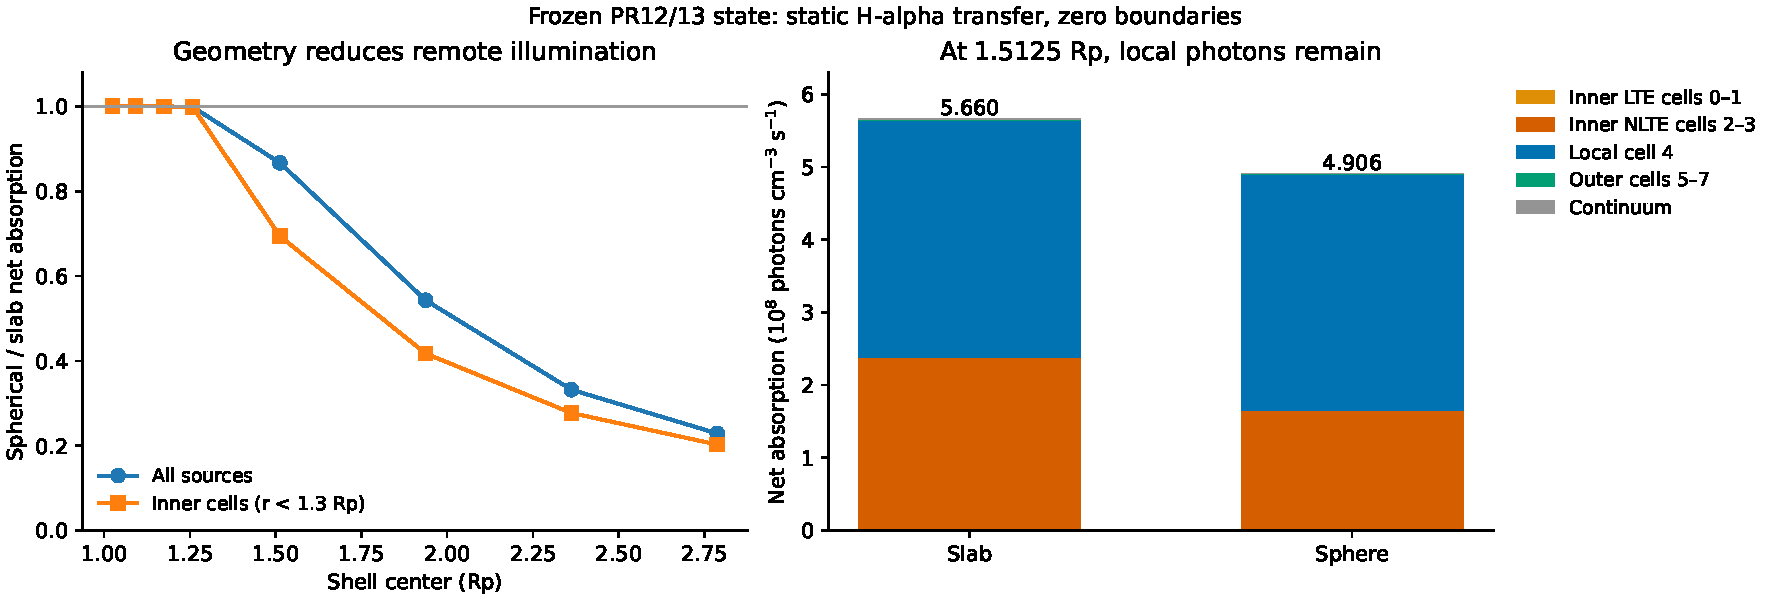
\includegraphics[width=\linewidth]{../mceg/evidence/halpha_geometry_effect_20261126/geometry_response.pdf}
 \caption{Static source-separated net absorption. The geometries retain
 identical local coefficients, not identical total emitting volumes.}
\end{figure}

The net radiative excitation changes more than the total absorption because
emission and absorption nearly cancel. Table~\ref{tab:rates} gives both.
Spherical geometry reduces the added-field net excitation by about $60\%$
relative to the slab, but the result remains positive. The \emph{same-state}
native escape/shielding closure instead gives
$-1.526\times10^7$ cm$^{-3}$\,s$^{-1}$ for the H$\alpha$ contribution to $n=3$.
Thus even the spherical resolved field gives more excitation than the original
closure. This is not evidence for a source-function reduction relative to that
original atmosphere.

\begin{table}[htbp]
\centering
\caption{Primary receiver rates in units of $10^8$ cm$^{-3}$\,s$^{-1}$.
The last column subtracts rest-frame spontaneous emission from all-source
absorption, except for the directly extracted native-closure row.}
\label{tab:rates}
\begin{tabular}{lrrr}
\toprule
Transfer case & Inner-source absorption & All-source absorption & Net excitation\\
\midrule
Native escape/shielding closure & --- & --- & $-0.1526$\\
Static slab & 2.3773 & 5.6600 & 1.2596\\
Static sphere & 1.6495 & 4.9058 & 0.5054\\
Sphere, saved radial flow & 1.6495 & 4.9054 & 0.5050\\
Sphere, upper flow $+5.5$ km/s & 1.6498 & 4.8985 & 0.4981\\
Sphere, upper flow $+13$ km/s & 1.6194 & 4.8465 & 0.4461\\
\bottomrule
\end{tabular}
\end{table}

\subsection{Velocity does not provide the required large suppression here}
Relative to the static sphere, the saved flow changes inner-source absorption
at the primary receiver by only $+0.00144\%$. Adding $5.5$ or $13$ km/s to all
upper cells changes it by $+0.0167\%$ and $-1.83\%$, respectively.
The corresponding net-excitation changes are $-0.0873\%$, $-1.445\%$ and
$-11.73\%$. These percentages do not describe equilibrium source functions.

The sign is not universal: with the actual flow, inner-source absorption at
$1.9375$, $2.3625$ and $2.7875R_p$ is $1.20$, $2.52$ and $5.72$ times the
static value. Optically thick source/receiver profiles and propagation select
frequencies differently from a two-Gaussian overlap estimate. The executed
transfer therefore does not support a universal Doppler suppression factor.

\subsection{Repeated conversion mostly recycles, rather than removes, photons}
Consider an inner-source H$\alpha$ photon already absorbed at the primary
receiver. The conditional spherical recycling network gives a $79.0087\%$
probability of ultimately leaving the outer boundary as H$\alpha$.
Deleting the real Ly$\beta$ decay branch as an isolation control changes this
to $79.0621\%$: only $0.0534$ percentage point. The control is not a physically
proposed atom.

\begin{table}[htbp]
\centering
\caption{Eventual outer H$\alpha$ probability, conditional on initial absorption
at $1.5125R_p$ and the specified reduced-network terminal exits.}
\begin{tabular}{lr}
\toprule
Network variation & Outer H$\alpha$ probability (\%)\\
\midrule
Coupled H$\alpha$/Ly$\beta$/O I network & 79.0087\\
Without the Ly$\beta$ spontaneous branch & 79.0621\\
Without O I resonance opacity & 79.0483\\
Without continuum absorption & 79.0696\\
Double continuum absorption & 78.9781\\
Without other H atomic exits & 93.1516\\
\bottomrule
\end{tabular}
\end{table}

There are about $40.7$ Ly$\beta$ emissions per initial absorbed H$\alpha$
photon, yet UV escape, UV continuum absorption and O I non-resonant cascades
together terminate only $0.134\%$ of these histories. Reverse recycling is
essential. The full-network outcome also includes $0.398\%$ H$\alpha$
continuum absorption, $1.014\%$ core loss, $1.509\%$ lower-state collisional
exits, $11.436\%$ other-shell excursions and $6.500\%$ ionization.
The last two are \emph{conditional exits}; subsequent recombination or cascades
can return radiation to H$\alpha$. They are not newly discovered irreversible
sinks and already have rates in the native atom.

This network uses positive lower-population absorption, unlike the net
extinction diagnostic in Table~\ref{tab:rates}. Stimulated photon multiplication
is omitted (the saved H$\alpha$ stimulated-to-absorption ratio reaches
$3.02\%$ in an inner cell and $0.463\%$ in the primary receiver).
O I collisional rates are at most $0.894\%$ of its radiative rates in the
tracked states and are omitted, as is O I photoionization.
Reabsorptions are redistributed uniformly within each coarse cell.
The reported survival probabilities are therefore conditional model diagnostics,
not complete atmospheric photon-destruction probabilities.

\subsection{Accuracy boundaries matter for the next coupled calculation}
Static photon accounting and source superposition close to better than
$10^{-9}$. Angle and spectral-density refinements change the reported static
absorption rates by less than $0.01\%$. Doubling the H$\alpha$ bandwidth
changes them by less than $0.008\%$, but changes the small, globally weighted
single-flight spherical outer escape fraction by $3.44\%$ relatively
($0.001672$ to $0.001730$). Its reliable description here is ``about $0.17\%$''.

The moving calculation agrees with the exact static solver at zero velocity
to about $3\times10^{-15}$ in $J$. For the strongest velocity probe, independent
angle, chord, spectral-density and bandwidth refinements change the primary
receiver's net excitation by less than $0.08\%$. No global moving flux or
photon-budget test is claimed. Crucially, the same bandwidth doubling changes
the small net residual in dense lower cell 1 by $105\%$, because much larger
absorption and emission terms cancel. This calculation does not establish
all-cell net-rate convergence for a coupled population solve.

The recycling calculation passes the recorded probability-balance and
primary-terminal refinement checks. Doubling the H$\alpha$ bandwidth changes
the primary outer H$\alpha$ probability by $0.127\%$ relatively;
the much smaller Ly$\beta$ on/off difference changes from $0.053397$ to
$0.053192$ percentage point (a $0.383\%$ relative change in the effect itself).
The joint angle, spectral-density and UV-wing control changes it by
$1.17\times10^{-6}$ relatively. The expected number of omitted electron or
Rayleigh scattering encounters over a recycled history is $1.90\times10^{-4}$,
which bounds the fraction of histories experiencing a first such encounter.
Detailed controls and limitations are retained in the conversion receipt.
These accuracy results support the
mechanism comparison at the specified receiver. They do not remove the
redistribution, coarse-cell or omitted cascade-return approximations.

The three tests point to the emitting region near $1.26R_p$ and its coupling
to the optically thick receiver as the next place to examine. Finite geometry
has a measurable effect; the saved velocity field and additional effective
loss through the tested Ly$\beta$/O I routes do not supply a large suppression
at this state. A consistent population response is needed before deciding
whether the observed brightness contrast improves.


\section{Verification and interpretation}
The numerical criteria are recorded in
\texttt{mceg/evidence/halpha\_coupling\_20261126/protocol.json}.
They include source superposition and photon balance, the static limit of
moving transfer, a common frequency/velocity shift control, finite-grid
refinements, normalized recycling probabilities and limiting cases.
The accompanying MCEG contract pins the actual source, equations and
compact numerical receipts. Historical atmosphere assessments and scientific
use requirements retain their previous status.

A reduction in Eq.~\eqref{eq:removal} is a mechanism-level result, not a
prediction that $n_3$, the source function, or the observed flux changes by
the same factor. The next population calculation must replace the selected
escape/shielding rates consistently with the new transport, retain collisional
and continuum rates, and recheck energy and population balance. Simply adding
the resolved field to already counted trapped radiation would double count
recycling. Only a new converged atmosphere rendered through the same
observation operator can establish improvement of the blue peak and trough.
\end{document}
